\documentclass{simple-paper}

\addbibresource{literature.bib}

% für etwas Beispieltext
\usepackage{lipsum}
%\usepackage{amsmath}

% ### Title

\title{Titel des Papers\\{\small Untertitel}}
\author{%
	\textsc{Autor 1}, \textsc{Autor 2}, \textsc{Autor 3}
}

\renewcommand{\journal}{Beispieljournal $\bullet$ 01/2021}

\renewcommand{\maketitlehookd}{%
\begin{abstract}
\noindent
% Abstract (1/3 Motivation, 1/3 Methode, 1/3 Ergebnisse)
Das Abstract gliedert sich zu jeweils $\frac{1}{3}$ in Hintergrund/Motivation/Problemstellung, Ansatz/Methodik sowie Ergebnisse und wissenschaftlicher Mehrwert.
\\
% Keywords
GPU-Programmierung, Parallelisierung, OpenMP, CUDA
\end{abstract}
}

\begin{document}

% Print the title{\tiny }
\maketitle

% Einzelne Kapitel einbinden
\section{Einführung}
How to configure Biber, the literature administration tool for Tex in TeXStudio, is shown in Fig.~\ref{fig:texStudio}.

\begin{figure*}[tb!]
	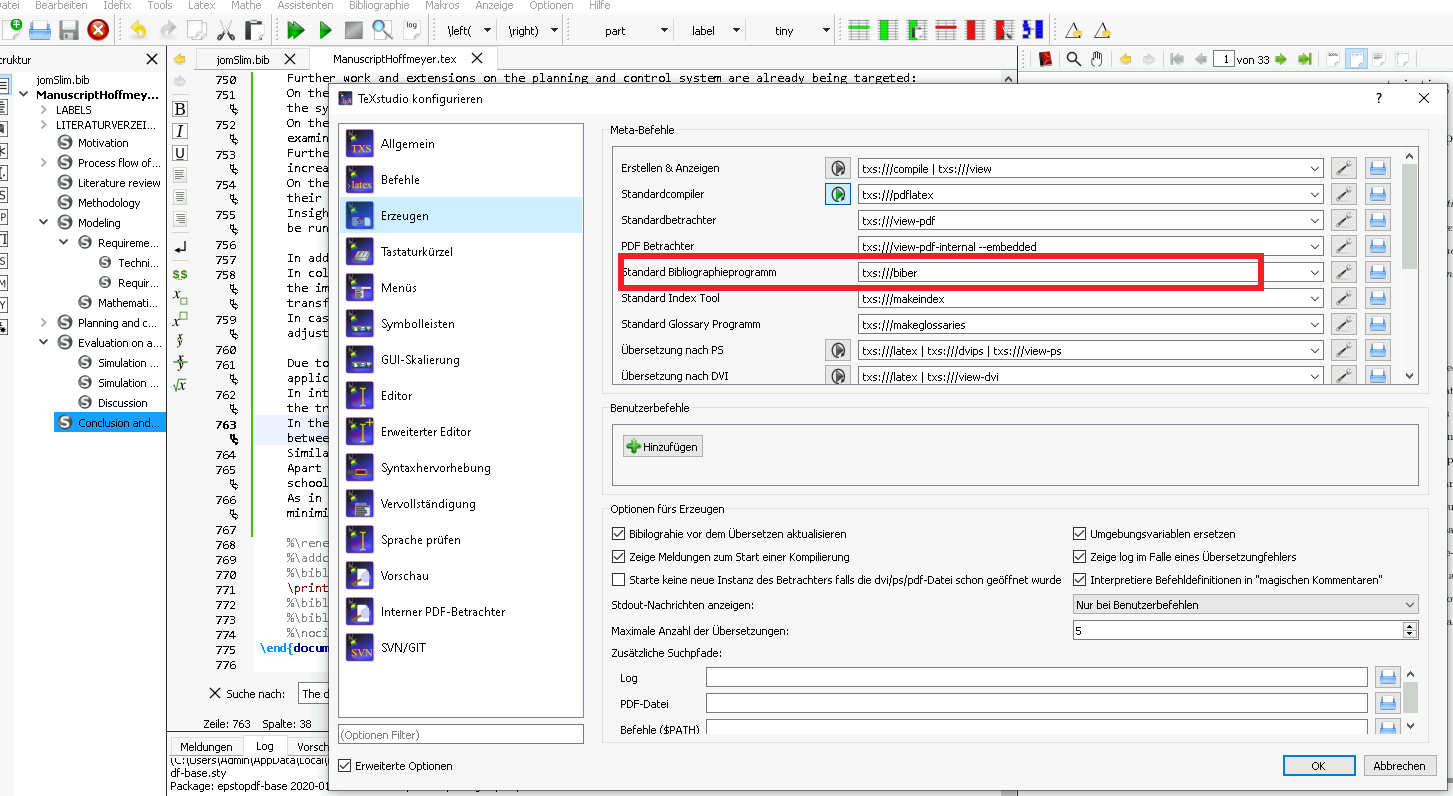
\includegraphics[width=\textwidth]{figures/texStudioConfigBiber}
	\caption{Bild über zwei Spalten, Konfiguration von Biber, der Literaturverwaltung in \LaTeX}
	\label{fig:texStudio}
\end{figure*}

\lipsum[1]


\section{Stand der Forschung}
In \textcite{Ernst2009} wird gezeigt, dass was \textcite{Bertsekas2005} bereits vorlegte, \lipsum[2-4]


\section{Vorgehen/Methodik}
\begin{figure*}[tb!]
	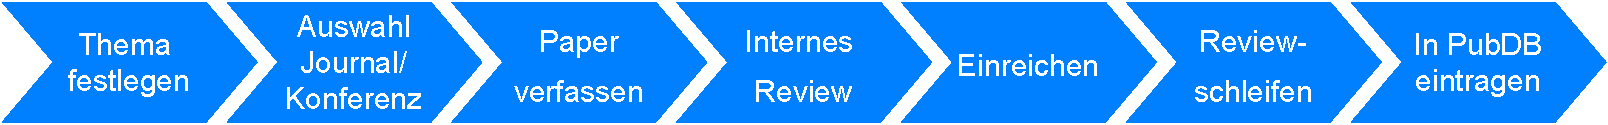
\includegraphics[width=\textwidth]{figures/paperflow_drawio.pdf}
	\caption{Ablauf des Paper Prozesses, über beide Spalten}
	\label{fig:process}
\end{figure*}

\lipsum[6]
In Figure~\ref{fig:process} the process of writing a paper is shown.

\begin{figure}[htb]
	\centering
	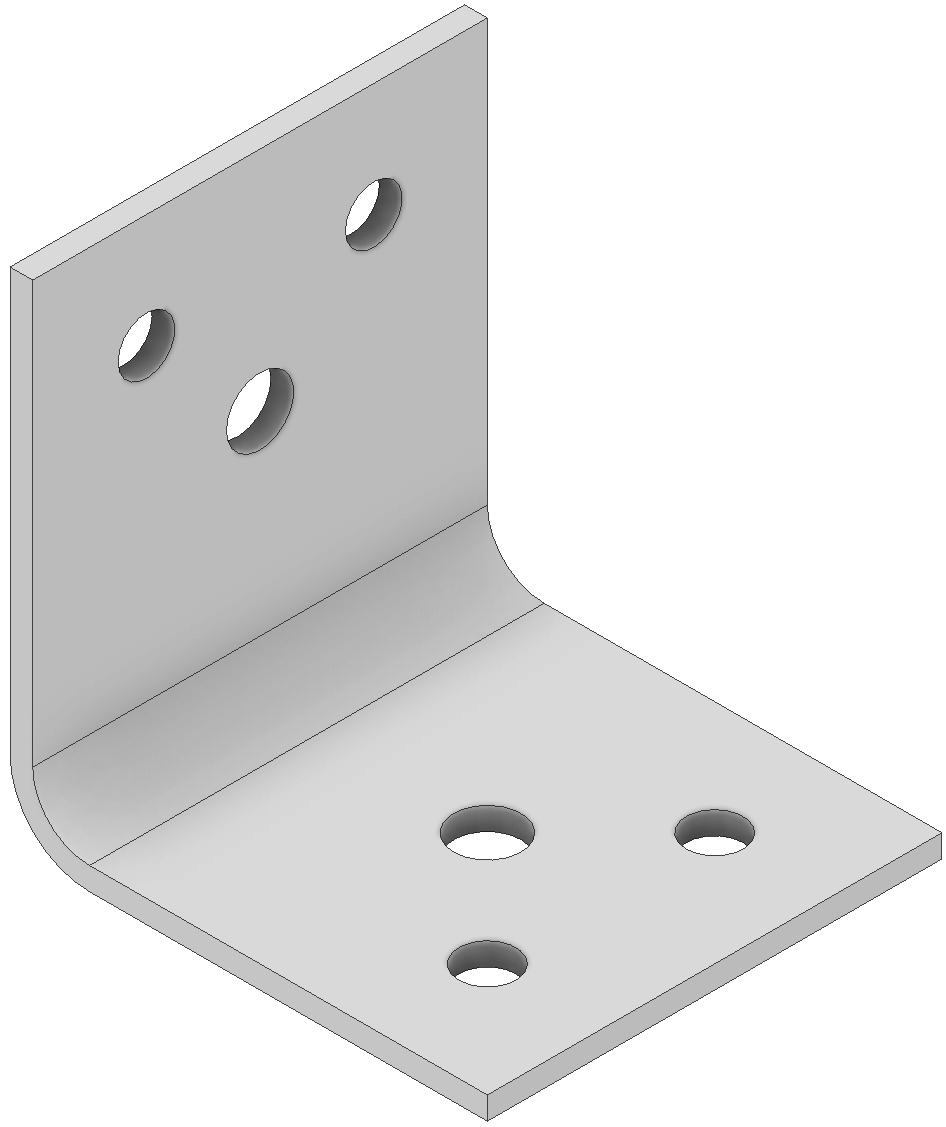
\includegraphics[width=.3\textwidth]{figures/example.jpg}
	\caption{Bildunterschrift für ein Bild mit 60\% der Textbreite (.5$\backslash$textwidth = Spaltenbreite)}
	\label{fig:example}
\end{figure}

\subsection{Unterüberschrift 1}
\lipsum[7]

\subsection{Unterüberschrift 2}
\lipsum[8]


\section{Ergebnisse}
The results are shown in Table~\ref{tab:results}. \lipsum[10]

\begin{table}[htb]
  \centering
  \begin{tabular}{lrr}
    \textbf{Scenario} & \textbf{KPI} & \textbf{Improvement}\\
    \hline
    Scenario 1 & 32.3 & -     \\
    Scenario 2 & 33.4 & 2\%   \\
    Scenario 3 & 38.6 & 10\%  \\
  \end{tabular}
  \caption{Results for the different scenarios}
  \label{tab:results}
\end{table}


\section{Diskussion/Fazit}
\lipsum[11]


\section*{Danksagung}
% vom Fördermittelgeber, Beispiel:
Das Forschungs- und Entwicklungsprojekt DPNB wird mit Mitteln des Bundesministeriums für Bildung und
Forschung (BMBF) im Programm „Innovationen für die Produktion, Dienstleistung und Arbeit von morgen“
(Förderkennzeichen 02P17D060 bis 02P17D066) gefördert und vom Projektträger Karlsruhe (PTKA) betreut.
Die Verantwortung für den Inhalt dieser Veröffentlichung liegt bei den Autoren.

\printbibliography

\vfill

\section*{Autorenangaben}
Autor 1, Autor 2\\
Hochschule Fulda – Fachbereich Elektrotechnik und Informationstechnik\\
Leipziger Straße 123\\
36037 Fulda\\
aut1@hs-fulda.de, aut2@hs-fulda.de\\

%Autor 3\\
%Fachbereich Produktionstechnik, Universität Bremen\\
%Badgasteiner Straße 1, 28359 Bremen\\
%Tel. +49 (0)421 / 218-50xxx\\
%aut3@biba.uni-bremen.de

\end{document}
